\chapter{引言}
\section{研究背景和意义}
地震勘探的终极目标是通过观测到地震数据来定量地估计地下模型。
弹性参数,包括纵(P)波速度,横(S)波速度以及密度等等物性参数可以通过岩石物理来定量的估计岩石物理参数,从而获得储层及其围岩的岩石性质。这对油气的开发,油田
监测以及CO$_2$注入等具有重要意义。传统的常规地震数据处理中,通常用声波方程来描述地震波在地下介质中的传播。而地下介质的真实模型往往要复杂得多,需要通过弹性
各向同性、具有垂直(水平)对称轴的横向各向同性(VTI,HTI)、正交各向异性(ORT)、衰减等等来更准确的描述波传播。但是模型假设越复杂,所引入的计算量也越大,
而所对应的多参数反问题也越困难。目前来看从声介质过渡到弹性介质能够以较小代价来获取较准确的模型近似。
尽管如此,从声波近似过渡到到弹性假设也会成倍地增加计算量,但是采用弹性波假设来进行成像或者反演仍然十分必要。因为考虑弹性假设的数据处理流程能区分数据中的
P波与S波模式,从而获得更多与岩性相关的信息,这对于岩性估计、流体识别、气云成像、裂缝与应力刻画以及密度估计都非常重要。
近年来,非常规油气藏,如致密页岩气(油)等开发技术极大地依赖于岩石物理参数的估计,这使得考虑弹性介质甚至各向异性假设都需要提上日程。

地震勘探中的诸多技术都非常依赖于速度模型的精度。
因此在众多物性参数中,如何获取准确的高分辨率速度模型是地震勘探中最为迫切的任务。
为了降低地震数据与模型描述之间的非线性程度,Claerbout(1985)\cite{Claerbout1985Imaging}在其书中将速度模型分解为两个部分:1)描述速度(阻抗)界面的高频部分;
2)描述波传播走时的低频部分。这样的分解方式分别对应于地震勘探中最核心的两个任务,也即偏移成像与速度建模。传统方法中偏移成像+AVO/AVA
技术通常用来获取模型的高频部分,
而偏移速度分析(MVA)和层析技术被用来恢复模型的低频部分。但是这类方法所能恢复的波数谱上存在明显的间断区域,正如著名的图\ref{fig:GapInSeisVel}
所示(选自Claerbout(1985)\cite{Claerbout1985Imaging}),速度模型的中低成分波数很难恢复。这就需要引入旨在恢复全频带速度信息的FWI方法。
而随着高性能计算能力的不断提升,基于波动理论来获取模型高、低波数成分的方法也受到了广泛关注。
\begin{figure}[!htb] 
   \centering 
   \subfloat[]{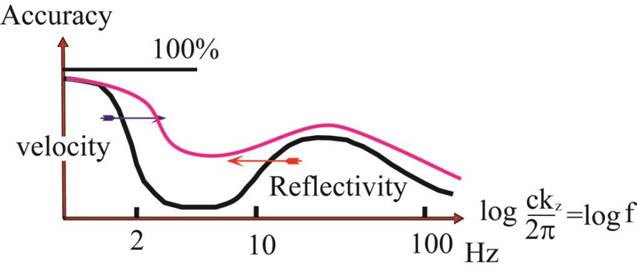
\includegraphics[width=0.68\textwidth]{Figure/chapter01/GapInSeis.jpg}}
   \caption{Vertical profiles of elastic WERTI and EFWI results at 1.4km (a) and
       3km (b). The black and blue lines indicate the true and linearly         increased
       initial model. The green and yellow lines indicate the WERTI and EFWI    results,
       respectively.
   }
   \label{fig:GapInSeisVel}
\end{figure}

传统常规方法中大多基于射线类方法进行成像与速度估计,这在模型复杂区域很难处理多路径以及焦散等问题。而基于波动方程的方法则可以避免上述问题。
目前基于波动理论的主要反演方法主要有以下三类:

1、FWI,该方法通过匹配数据中携带的所有信息,包括走时、振幅、模式转换、多次波等等,来获得对地下模型的全波数谱的
恢复。
相比走时反演和MVA,它可以获取更高分辨率的地下模型。
因此自从Lailly(1983)\cite{lailly1983seismic}和Taratola(1984)\cite{tarantola1984}建立了FWI理论框架之后,随着宽频带,宽方位数据采集的成熟,FWI
被认为是填补速度模型中尺度波数成分空白的最强有力的工具。
但是FWI也受到众多的制约,如强烈的非线性程度(cycle-skipping),数据不完备导致的有限观测孔径,地下实际介质的非弹性以及各向异性,计算代价十分昂贵等等,因此
FWI虽经过数十年发展所面临的挑战依然十分艰巨;

2、波动方程偏移速度分析(WEMVA),该类方法旨在更新模型中的长波长背景速度,也即模型的低波数成分。
目前主流的做法通常利用数据中的反射波信息,通过获取反射波波路径信息来获得模型中深部的速度更新。
而根据其目标函数的残差类型又可以分为数据域反演(如Xu et al., 2012\cite{xu:2012};Wu and Alkhalifah, 2015\cite[]{Wu2015}; Zhou et al, 
2015\cite[]{zhou:2015}; Chi et al, 2015\cite{chi:2015})和扩展成像域反演(如Sava和Fomel, 2006\cite{Sava2006}; Almomin和Biondi, 2012\cite{Almomin2012})。
此类方法与基于射线理论的成像域层析与数据域(非线性)层析方法一脉相承,但是避免了传统层析流程中繁琐的人工拾取工作,不过其同样也会受困于cycle-skipping等问题;

3、最小二乘逆时偏移(LSRTM),该方法可以看作是线性化的FWI,在初始模型足够好的时候通过匹配模拟数据与观测数据的振幅来获得地下反射系数模型。常规偏移成像
采用伴随算子来近似正传算子的伪逆,从而近似地获得反射率的成像结果。但是伴随算子通常近似效果很差,最小平方偏移(LSM)通过迭代方式来获取正传算子的伪逆从而获得
更好的成像效果((Nemeth et al., 1999,Kühl and Sacchi, 2003,Dai, 2012)。该过程可以看作是对目标函数对模型的二阶导数,也即Hessian,近似求逆的过程。

结合以上背景,如何恢复弹性介质中的速度模型将对勘探地球物理的发展至关重要。将弹性假设引入到以上反演问题中将会大大增加反问题的非线性程度。同时,多参数反演
也会带来参数间的耦合效应,这会进一步增加反演难度。由于计算机能力提升、多分量观测数据的增多以及解决声波FWI无法回避的问题的需要,考虑弹性甚至各向异
性的全波形反演逐渐成为研究热点。弹性波多分量数据中同时含有P波和S波,这两种不同波模式对地下介质有着不同的刻画作用。
近年来弹性波波模式分离技术能够提供准确的P或S波数据子集,这对反演中采取更多的多尺度策略带来可能性。在反演过程中,不同参数采用不同的数据子集或者不同的反演阶段
采用不同的数据子集,这将大大降低法多参数反演的非线性程度,同时也可以回避参数间的耦合效应。在本文中,这种策略将贯穿始终,
模式解耦将在EFWI,弹性波波动放程反射走时反演(EWERTI)以及E-LSRTM中提供的分离的P或S波数据,来帮助获得更好的反演结果。
\section{研究现状}
\subsection{弹性波FWI研究现状}
\subsection{弹性反射波FWI研究现状}
\subsection{弹性波LSRTM研究现状}
\section{研究内容}
